\documentclass[10pt]{beamer}
\usetheme{Boadilla} %CHANGE THIS FOR DIFFERENT COLOR ETC.
\usepackage{xcolor, soul}
\sethlcolor{red}
\usepackage[absolute,overlay]{textpos}
\usepackage[ruled,vlined]{algorithm2e}
\usepackage{dsfont}
\usepackage{array}
\usepackage{tikz}
\usetikzlibrary{shapes, arrows.meta, positioning}
\usepackage[style=alphabetic]{biblatex}  
\addbibresource{lib.bib}
\usepackage{caption}
\usepackage{xcolor}
\usepackage{mathrsfs}
\usepackage{mathtools}
\usepackage{comment}



\newtheoremstyle{reminder}% Custom style for reminders
  {3pt} % Space above
  {3pt} % Space below
  {\itshape} % Body font
  {} % Indent amount
  {\bfseries\color{blue}} % Theorem head font
  {.} % Punctuation after theorem head
  {.5em} % Space after theorem head
  {} % Theorem head spec (can be left empty, meaning `normal`)

\theoremstyle{reminder}
\newtheorem{reminder}{Reminder}

\author[Jonas Müller]{Jonas Müller}

\setbeamertemplate{enumerate item}{\arabic{enumi}.}  % Use regular numbers and a period

%%%%%%%%%%%%%%%%%% Begin of the Presentation %%%%%%%%%%%%%%%%%

\begin{document}

\title[Physics Informed Diffusion Models]{Physics Informed Diffusion Models}
\institute{}
\date{}

\begin{frame}
    \titlepage
\end{frame}

%%%%%%%%%%%%%%%%%% Outline %%%%%%%%%%%%%%%%%%%%%
\section{Recap Diffusion Models}

\section{Setup: Physics Informed Diffusion Models}

\section{Training Algorithm}

\section{Experiments}
\section{Discussion}

\begin{frame}
    \frametitle{Outline}
    \tableofcontents
\end{frame}

%%%%%%%%%%%%%%%%%% Beginning of slides %%%%%%%%%%%%%%%%%

\begin{frame}{Recap Diffusion Models}
    \begin{itemize}
        \item First point
        \item Second point
        \item Third point
    \end{itemize}
\end{frame}

\begin{frame}{Physics Informed Diffusion Models}
    \begin{definition}
        We assume our physics is described by a PDE on $\Omega \subseteq \mathbb{R}^d$ of the form 
        \[
            \mathcal{F}\left(u(\xi)\right) = 0 \quad \text{with} \quad \xi \in \Omega. 
        \]
        and we have a boundary operator 
        \[\mathcal{B}\left(u(\xi)\right) = 0 \quad \text{with} \quad \xi \in \partial \Omega.\]
        where $u : \Omega \rightarrow \mathbb{R}^c$ is the solution of interest. To simplify, we write \[R(u(\xi)) = [\mathcal{F}(u(\xi)), \mathcal{B}(u(\xi))]^\top\].
    \end{definition}
    They only consider $$[1,...,n] \times [1,...,n] \subseteq \mathbb{Z}_n \times \mathbb{Z}_n.$$
    Similar to standard image based diffusion models, data is then considered to be given as $x_0 \in \mathbb{R}^{c \times n \times n}$ and $\mathcal{F}, \mathcal{B}$ are discretized accordingly.
\end{frame}



\begin{frame}{Setting up Physics based Training Objective}
    The residual $\mathcal{R} = 0$ in the non discrete gives us an infinite amount of information. 
    To utilize this, we introduce a loss based on $\mathcal{R}$ via a \textit{virtual observable}.

    $$q_{\mathcal{R}}(\cdot \mid x_0) \sim \mathcal{N}(\mathcal{R}(x_0), \sigma^2 I_d)$$


    \begin{definition}
        Define $$p_\theta(\hat{r}) = \int_{\Omega} q_{\mathcal{R}}(\hat{r} \mid x_0) p_\theta(x_0) dx_0$$
        then we can optimize 
        $$ \arg \max_\theta \mathbb{E}_{\hat{r} \sim \delta_0}\left[\log p_\theta(\hat{r})\right]=\arg \max _\theta \mathbb{E}_{x_0 \sim p_\theta}\left[\log q_{\mathcal{R}}\left(\hat{r}=0 \mid x_0\right)\right] .$$
    \end{definition}
    So we can train our model by evaluating $x_0$ on the the virtual observable log likelihood.
    Note that this loss is equivalent to $$\arg \max_\theta \log p_\theta(0) = \arg \max _\theta \mathbb{E}_{x_0 \sim p_\theta}\left[\log q_{\mathcal{R}}\left(0 \mid x_0\right)\right]$$
\end{frame}

\begin{frame}
\begin{figure}[h]
\centering
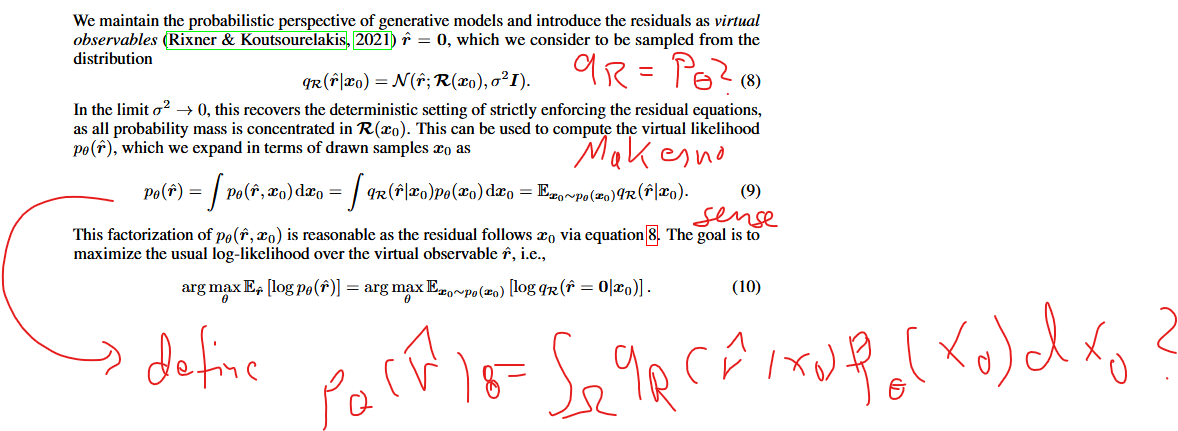
\includegraphics[width=0.8\linewidth]{images/2026-01-06-00-39-43.png}
\caption{}
\label{fig:main-2026-01-06-00-39-43}
\end{figure}
\end{frame}

\begin{frame}{Introducing the Data Loss}
    
\end{frame}

\begin{frame}{Full Training Algorithm}
    
\end{frame}

\begin{frame}{Discussion}
    \begin{itemize}
        \item They only consider 2d data and PDEs on $\mathbb{R}^2$, how this works on higher dimensions is not tested. 
    \end{itemize}
\end{frame}


%%%%%%%%%%%%%%%%%% End of Presentation %%%%%%%%%%%%%%%%%

\end{document}